\documentclass[UTF8,fontset=none,12pt]{ctexart}

\setCJKmainfont{Songti SC}
\setCJKsansfont{PingFang SC}
\setCJKmonofont{PingFang SC}

\usepackage[a4paper,margin=2.35cm]{geometry}
\usepackage{amsmath,amssymb,amsthm,mathtools,bm}
\usepackage{graphicx}
\usepackage{float}
\usepackage{booktabs}
\usepackage{enumitem}
\usepackage[hidelinks]{hyperref}

\newcommand{\C}{\mathbb{C}}
\newcommand{\R}{\mathbb{R}}
\newcommand{\range}{\operatorname{range}}
\newcommand{\nullspace}{\operatorname{null}}
\newcommand{\rank}{\operatorname{rank}}
\newcommand{\Span}{\operatorname{span}}
\theoremstyle{definition}
\newtheorem{theorem}{定理}
\renewcommand{\thetheorem}{6.\arabic{theorem}}

\title{数值线性代数\quad 第 6 讲：投影算子}
\author{Lloyd N. Trefethen、David Bau III\quad 中文阅读版}
\date{}

\begin{document}
\maketitle
\pagestyle{plain}

我们现在进入全书第二部分，主题是正交性.本讲从投影矩阵（也称投影算子）这一基本工具开始，同时讨论正交投影与非正交投影.

\section*{投影算子}

投影算子是满足
\begin{equation}
    P^2=P
    \tag{6.1}
\end{equation}
的方阵.这样的矩阵也称为\textbf{幂等矩阵}. 这个定义既包含下面将讨论的正交投影，也包含非正交投影.为了避免混淆，非正交情形也可以称为\textbf{斜投影算子}.

“投影”这个术语可以这样理解：设想从恰当的方向把光照向子空间 $\range(P)$，那么向量 $v$ 在这个子空间上的投影 $Pv$ 就像是它投下的影子.下面暂时沿用这个物理图像.

如果 $v\in\range(P)$，那么 $v$ 恰好位于自己的影子上，应用投影算子后仍得到 $v$.确实，若 $v=Px$，则
\[
    Pv=P^2x=Px=v.
\]
当 $v\ne Pv$ 时，光线从什么方向照来？一般而言，答案取决于 $v$；但对给定的 $v$，只需画出从 $v$ 指向 $Pv$ 的线段，其方向由 $Pv-v$ 给出（见图~\ref{fig:oblique}）.把投影算子作用到这个方向上，可得
\[
    P(Pv-v)=P^2v-Pv=0.
\]
因此
\[
    Pv-v\in\nullspace(P).
\]
换言之，对不同的 $v$，光线方向可能不同，但它总由 $\nullspace(P)$ 中的向量描述.

    \begin{figure}[H]
    \centering
    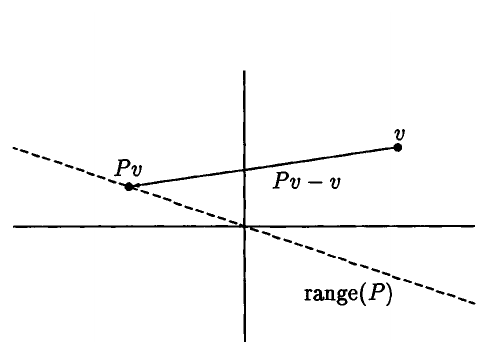
\includegraphics[width=0.55\linewidth]{../assets/figure-6-1.png}
    \caption{斜投影. 图中的 $Pv-v$ 属于 $\nullspace(P)$，而 $Pv$ 位于 $\range(P)$.}
    \label{fig:oblique}
\end{figure}

\section*{互补投影算子}

如果 $P$ 是投影算子，那么 $I-P$ 也是投影算子，因为它同样幂等：
\[
    (I-P)^2=I-2P+P^2=I-P.
\]
矩阵 $I-P$ 称为 $P$ 的\textbf{互补投影算子}.

$I-P$ 投影到哪个空间？正好是 $P$ 的零空间.首先，如果 $Pv=0$，那么 $(I-P)v=v$，所以
\[
    \range(I-P)\supseteq\nullspace(P).
\]
反过来，对任意 $v$，都有 $(I-P)v=v-Pv\in\nullspace(P)$，因此
\[
    \range(I-P)\subseteq\nullspace(P).
\]
于是，对任意投影算子 $P$，
\begin{equation}
    \range(I-P)=\nullspace(P).
    \tag{6.2}
\end{equation}
把 $P$ 写成 $P=I-(I-P)$，可得到互补结论
\begin{equation}
    \nullspace(I-P)=\range(P).
    \tag{6.3}
\end{equation}

我们还可以看出
\[
    \nullspace(I-P)\cap\nullspace(P)=\{0\};
\]
因为同时属于这两个空间的向量 $v$ 满足
\[
    v=v-Pv=(I-P)v=0.
\]
等价地，
\begin{equation}
    \range(P)\cap\nullspace(P)=\{0\}.
    \tag{6.4}
\end{equation}

这些计算说明，投影算子把 $\C^m$ 分解为两个空间.反过来，设 $S_1$ 和 $S_2$ 是 $\C^m$ 的两个子空间，满足
\[
    S_1\cap S_2=\{0\},\qquad S_1+S_2=\C^m,
\]
其中 $S_1+S_2$ 表示由 $S_1$ 与 $S_2$ 张成的空间，即所有形如 $s_1+s_2$（$s_1\in S_1$、$s_2\in S_2$）的向量组成的集合.这样的一对空间称为\textbf{互补子空间}.此时存在投影算子 $P$，使得
\[
    \range(P)=S_1,\qquad \nullspace(P)=S_2.
\]
我们称 $P$ 为沿着 $S_2$ 投影到 $S_1$ 的投影算子.

这个投影算子及其互补投影可以看作下列问题的唯一解：

\begin{quote}
给定 $v$，求 $v_1\in S_1$ 与 $v_2\in S_2$，使得 $v_1+v_2=v$.
\end{quote}

投影 $Pv$ 给出 $v_1$，互补投影 $(I-P)v$ 给出 $v_2$.这两个向量之所以唯一，是因为所有解都可写成
\[
    (Pv+v_3)+((I-P)v-v_3)=v,
\]
而 $v_3$ 必须同时属于 $S_1$ 与 $S_2$，所以只能有 $v_3=0$.

投影算子及其互补投影的一个熟悉应用来自特征向量展开.设 $m\times m$ 矩阵 $A$ 有一组完备的特征向量 $\{v_j\}$，如式 (5.1) 中那样；也就是说，$\{v_j\}$ 构成 $\C^m$ 的一组基.我们经常关心向量在这组基下的展开.例如，给定 $x\in\C^m$，它沿某个特定特征向量 $v$ 的分量是什么？答案是 $Px$，其中 $P$ 是某个秩一投影算子.不过，我们暂不展开这一细节，转而讨论本书主要关注的一类投影算子.

\section*{正交投影算子}

正交投影（见图~\ref{fig:orthogonal}）是沿着子空间 $S_2$ 投影到子空间 $S_1$，且 $S_1$ 与 $S_2$ 正交的投影算子.注意：正交投影算子不是正交矩阵！

\begin{figure}[H]
    \centering
    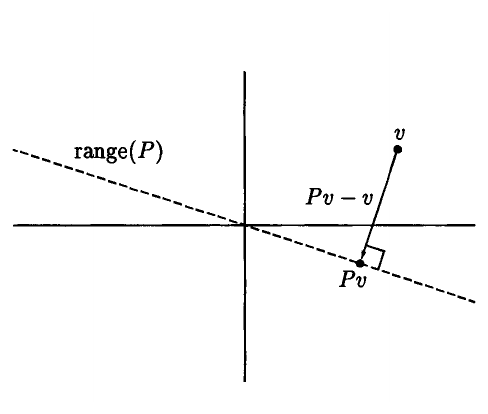
\includegraphics[width=0.55\linewidth]{../assets/figure-6-2.png}
    \caption{正交投影. 此时 $Pv-v$ 垂直于 $\range(P)$.}
    \label{fig:orthogonal}
\end{figure}

正交投影还有一个代数定义：它是同时满足式 (6.1) 与
\[
    P^*=P
\]
的厄米投影算子.当然，我们需要证明这两个定义等价.

\begin{theorem}
投影算子 $P$ 是正交投影算子，当且仅当 $P=P^*$.
\end{theorem}

\begin{proof}
若 $P=P^*$，则取 $Px\in S_1$ 与 $(I-P)y\in S_2$，有
\[
    x^*P^*(I-P)y=x^*(P-P^2)y=0.
\]
所以这两个空间正交，投影算子确实是正交的.

下面证明“只有当”方向.设 $P$ 沿 $S_2$ 投影到 $S_1$，其中 $S_1\perp S_2$，且 $S_1$ 的维数为 $n$.可以如下构造 $P$ 的 SVD：取 $\C^m$ 的一组标准正交基 $\{q_1,q_2,\ldots,q_m\}$，其中 $\{q_1,\ldots,q_n\}$ 是 $S_1$ 的基，$\{q_{n+1},\ldots,q_m\}$ 是 $S_2$ 的基.对 $j\le n$，有 $Pq_j=q_j$；对 $j>n$，有 $Pq_j=0$.

令 $Q$ 为以 $q_j$ 为第 $j$ 列的酉矩阵，则
\[
    Q^*PQ=\Sigma=\operatorname{diag}(I_n,0).
\]
这是一个对角矩阵，其前 $n$ 个对角元为 1，其余对角元为 0.因此我们构造出了 $P$ 的奇异值分解
\begin{equation}
    P=Q\Sigma Q^*.
    \tag{6.5}
\end{equation}
（注意，这同时也是特征值分解 (5.1).）于是
\[
    P^*=(Q\Sigma Q^*)^*=Q\Sigma^*Q^*=Q\Sigma Q^*=P,
\]
因为 $\Sigma$ 是实对角矩阵.
\end{proof}

\section*{用标准正交基进行投影}

除平凡情形 $P=I$ 外，正交投影都有一些等于零的奇异值.因此，自然的做法是删去式 (6.5) 中 $Q$ 的“沉默列”，使用约化 SVD 而不是完整 SVD.于是得到极其简洁的表达式
\begin{equation}
    P=\widehat Q\widehat Q^*,
    \tag{6.6}
\end{equation}
其中 $\widehat Q$ 的列向量是标准正交的.

在式 (6.6) 中，矩阵 $\widehat Q$ 不一定来自 SVD.设 $\{q_1,\ldots,q_n\}$ 是 $\C^m$ 中任意一组标准正交向量，$\widehat Q$ 是以它们为列的 $m\times n$ 矩阵.由式 (2.7)，任意 $v\in\C^m$ 都可以分解为列空间分量与正交分量：
\[
    v=r+\sum_{i=1}^n(q_iq_i^*)v.
\]
因此映射
\begin{equation}
    v\longmapsto\sum_{i=1}^n(q_iq_i^*)v
    \tag{6.7}
\end{equation}
是到 $\range(\widehat Q)$ 上的正交投影.用矩阵写就是
\[
    y=\widehat Q\widehat Q^*v.
\]
只要 $\widehat Q$ 的列是标准正交的，乘积 $\widehat Q\widehat Q^*$ 就一定是到 $\widehat Q$ 列空间上的投影算子，与 $\widehat Q$ 是如何得到的无关.它可以来自把单位矩阵的一个完整分解
\[
    v=QQ^*v
\]
中的某些列和行删去，也可以来自完全不同的构造.

正交投影的互补投影仍是正交投影，因为 $I-\widehat Q\widehat Q^*$ 是厄米矩阵.这个互补投影投影到与 $\range(\widehat Q)$ 正交的空间.

\newpage
正交投影的一个重要特例，是提取单个方向分量的秩一正交投影.对单位向量 $q$，它写成
\begin{equation}
    P_q=qq^*.
    \tag{6.8}
\end{equation}
这些秩一投影就是构造高秩投影的基本部件，如式 (6.7) 所示.它们的互补投影消去 $q$ 方向上的分量，是秩为 $m-1$ 的正交投影：
\begin{equation}
    P_{\perp q}=I-qq^*.
    \tag{6.9}
\end{equation}

式 (6.8) 与 (6.9) 假设 $q$ 是单位向量.对任意非零向量 $a$，相应公式为
\begin{equation}
    P_a=\frac{aa^*}{a^*a},
    \tag{6.10}
\end{equation}
以及
\begin{equation}
    P_{\perp a}=I-\frac{aa^*}{a^*a}.
    \tag{6.11}
\end{equation}

\section*{用任意基进行投影}

从任意基出发，即使基向量不正交，也可以构造 $\C^m$ 的某个子空间上的正交投影.设子空间由线性无关向量 $\{a_1,\ldots,a_n\}$ 张成，令 $A$ 为以这些向量为列的 $m\times n$ 矩阵.

把 $v$ 正交投影到 $\range(A)$ 得到 $y$ 时，差向量 $y-v$ 必须与 $\range(A)$ 正交.这等价于：对每个 $j$，都有
\[
    a_j^*(y-v)=0.
\]
由于 $y\in\range(A)$，可写成 $y=Ax$，于是
\[
    a_j^*(Ax-v)=0
\]
对每个 $j$ 成立；等价地，
\[
    A^*(Ax-v)=0,\qquad A^*Ax=A^*v.
\]
容易证明，因为 $A$ 满列秩，$A^*A$ 非奇异（见习题 6.3）.因此
\begin{equation}
    x=(A^*A)^{-1}A^*v.
    \tag{6.12}
\end{equation}
最后，投影向量 $y=Ax$ 为
\[
    y=A(A^*A)^{-1}A^*v.
\]
所以到 $\range(A)$ 上的正交投影可以写成
\begin{equation}
    P=A(A^*A)^{-1}A^*.
    \tag{6.13}
\end{equation}
注意，这是式 (6.10) 的多维推广.当 $A=\widehat Q$ 且列向量标准正交时，括号中的项退化为单位矩阵，从而恢复式 (6.6).

\section*{习题}

\begin{enumerate}[label=\textbf{6.\arabic*.},leftmargin=*]
    \item 若 $P$ 是正交投影算子，证明 $I-2P$ 是酉矩阵，并给出一个几何解释.
    \item 设 $E$ 是提取 $m$ 维向量“偶部”的 $m\times m$ 矩阵：
    \[
        Ex=\frac{x+Fx}{2},
    \]
    其中 $F$ 是把 $(x_1,\ldots,x_m)^*$ 翻转为 $(x_m,\ldots,x_1)^*$ 的 $m\times m$ 矩阵.$E$ 是正交投影、斜投影，还是根本不是投影？它的元素是什么？
    \item 给定 $A\in\C^{m\times n}$ 且 $m\ge n$，证明 $A^*A$ 非奇异，当且仅当 $A$ 满秩.
    \item 考虑矩阵
    \[
        A=\begin{bmatrix}1&0\\0&1\\1&0\end{bmatrix},
        \qquad
        B=\begin{bmatrix}1&2\\0&1\\1&0\end{bmatrix}.
    \]
    请手算回答：
    \begin{enumerate}[label=(\alph*),leftmargin=2em]
        \item 到 $\range(A)$ 上的正交投影 $P$ 是什么？向量 $(1,2,3)^*$ 在 $P$ 下的像是什么？
        \item 对 $B$ 回答同样的问题.
    \end{enumerate}
    \item 设 $P\in\C^{m\times m}$ 是非零投影算子.证明 $\lVert P\rVert_2\ge 1$，且等号成立当且仅当 $P$ 是正交投影算子.
\end{enumerate}

\end{document}
